\documentclass[11pt,a4paper]{article}

% ----------------------------------------------------------------- packages
\usepackage[utf8]{inputenc}
\usepackage[T1]{fontenc}
\usepackage{lmodern}
\usepackage[a4paper,margin=2.3cm]{geometry}
\usepackage{amsmath,amssymb}
\usepackage{graphicx}
\usepackage{booktabs}
\usepackage{caption}
\usepackage{float}
\usepackage{xcolor}
\usepackage{enumitem}
\usepackage{array}
\usepackage{makecell}
\usepackage{fancyhdr}
\usepackage[hidelinks]{hyperref}

\graphicspath{{figures/}{report/figures/}}
\captionsetup{font=small,labelfont=bf}
\definecolor{accent}{HTML}{1F3A93}
\definecolor{lightgray}{HTML}{F0F0F0}

\pagestyle{fancy}
\fancyhf{}
\lhead{\small SAAM Project 2026 -- Group BR}
\rhead{\small Portfolio Allocation with a Carbon Objective}
\cfoot{\small\thepage}
\renewcommand{\headrulewidth}{0.4pt}

\newcommand{\pmv}{$P^{(mv)}_{oos}$}
\newcommand{\pvw}{$P^{(vw)}$}
\newcommand{\pmvh}{$P^{(mv)}_{oos}(0.5)$}
\newcommand{\pvwh}{$P^{(vw)}_{oos}(0.5)$}
\newcommand{\pnz}{$P^{(vw)}_{oos}(NZ)$}
\newcommand{\co}{CO\textsubscript{2}}

% ----------------------------------------------------------------- title
\title{\vspace{-1.2cm}\Large\bfseries Sustainability Aware Asset Management\\[2pt]
\large Portfolio Allocation with a Carbon Emission Reduction Objective}
\author{\normalsize Group BR \quad$\vert$\quad North America + Europe \quad$\vert$\quad
Scope 1 + Scope 2}
\date{\normalsize May 2026}

\begin{document}
\maketitle
\thispagestyle{fancy}
\vspace{-0.7cm}

% ================================================================ summary
\begin{center}
\colorbox{lightgray}{%
\begin{minipage}{0.96\textwidth}
\vspace{4pt}
\textbf{Executive summary.} We build five long-only equity portfolios on a
universe of North American and European firms and back-test them monthly from
January 2014 to December 2024. The value-weighted benchmark (\pvw) delivers a
Sharpe ratio of 0.72; the global minimum-variance portfolio (\pmv) reaches only
0.42 and, strikingly, carries a carbon footprint roughly five times larger than
the benchmark -- low-volatility investing is, in this universe, an implicit bet
on carbon-heavy regulated utilities. Adding a carbon constraint is cheap for the
\emph{passive} investor: cutting the footprint by 50\% through a tracking-error
overlay (\pvwh) costs 0.03 of Sharpe ratio and 1.1\% annual tracking
error, and a 10\%-per-year net-zero glide path (\pnz) costs barely more. For the
\emph{active} minimum-variance investor, halving the footprint (\pmvh) is not a
cost at all: it trims concentrated, carbon-intensive positions and slightly
\emph{improves} both volatility and Sharpe ratio. Decarbonisation, properly
implemented, is close to a free lunch over this sample.
\vspace{4pt}
\end{minipage}}
\end{center}

\vspace{0.2cm}

% ================================================================ 1
\section{Introduction}

This project implements the climate-aware asset-management concepts of the
course on a concrete allocation problem. Group BR is assigned the
\textbf{North America + Europe} region and the \textbf{Scope 1 + Scope 2}
emission perimeter. The work proceeds in two parts.

\textbf{Part I} builds two reference portfolios: the value-weighted benchmark
\pvw{} and the long-only global minimum-variance portfolio \pmv. \textbf{Part II}
adds a carbon objective and constructs three decarbonised portfolios: a
minimum-variance portfolio whose footprint is capped at 50\% of \pmv{}
(\pmvh), a tracking-error-minimising portfolio whose footprint is capped at
50\% of the benchmark (\pvwh), and a net-zero portfolio whose footprint is cut
cumulatively by 10\% per year (\pnz).

All empirical work is carried out in Python; the accompanying notebook
\texttt{SAAM\_Project\_2026.ipynb} reproduces every table and figure of this
report when run from top to bottom.

\paragraph{Sample convention.} The data span end-1999 to end-2025. Following the
instructor's consistency note, the first allocation is decided in
December~2013 and the last in December~2023; portfolio performance is then
measured month by month from January~2014 to December~2024, giving
$T=132$ monthly observations. Stopping in December~2024 keeps the
back-test comparable across groups and avoids the incomplete 2025 window.

% ================================================================ 2
\section{Data and Cleaning}

\subsection{Datasets}

The raw Datastream files cover 2{,}545 firms worldwide. Filtering on the
assigned region (\texttt{AMER} and \texttt{EUR}) leaves 1{,}302 firms. For each
firm we use the monthly total-return index $P_{i,t}$ and monthly market
capitalisation $Cap_{i,t}$, and the annual series of Scope~1 and Scope~2 \co{}
emissions $E_{i,Y}$ (tonnes), revenues $Rev_{i,Y}$ (thousand USD) and year-end
market capitalisation. The one-month risk-free rate is taken from the provided
file and converted to a monthly decimal.

\subsection{Cleaning rules}

We apply the cleaning rules of the project statement:
\begin{itemize}[nosep,leftmargin=1.3em]
  \item \textbf{Unmatched ISINs.} Columns that are entirely empty are dropped
        from all tables (Datastream could not match the security).
  \item \textbf{Low prices.} Any total-return-index value below 0.5 is set to
        missing, because returns computed from near-zero prices explode.
  \item \textbf{Delistings.} When a firm's last valid price is followed by
        missing values, we book a realised return of $-100\%$ in the
        following month. This rule flags \textbf{112} delistings over the
        sample, so that defaults are correctly penalised rather than silently
        dropped.
  \item \textbf{Missing carbon / revenue.} Emissions and revenues are
        forward-filled across years: a gap in the middle or at the end of the
        sample is replaced by the most recent available figure. A firm with no
        figure at all before year $Y$ cannot be held in year $Y+1$.
\end{itemize}
Returns are simple monthly returns, $R_{i,t}=P_{i,t}/P_{i,t-1}-1$.

\subsection{Investment set}

At the end of each year $Y$ we define the set of firms that may be held in
year $Y+1$. A firm enters the investment set if it (i)~belongs to the assigned
region, (ii)~has at least 36 monthly returns over the 10-year estimation
window, (iii)~shows at most 50\% stale (exactly-zero) returns over that window,
(iv)~has a valid year-end price and market capitalisation, and (v)~has carbon
\emph{and} revenue data available. Criterion~(iii) removes illiquid stocks
whose artificially low volatility would otherwise attract excessive weight;
criterion~(v) guarantees that the carbon footprint and intensity are defined
for \emph{every} firm, so that the \textbf{same investment set is used by all
five portfolios}, as required for a clean comparison between Parts~I and~II.
Table~\ref{tab:set} reports the resulting set sizes.

\begin{table}[H]
\centering
\caption{\textbf{Investment set size by allocation year.} Number of firms
satisfying all eligibility criteria at the end of year $Y$, i.e.\ the firms that
may be held over year $Y+1$. The set grows over time as carbon-data coverage
improves; this is the common universe for all five portfolios.}
\label{tab:set}
\small
\begin{tabular}{lccccccccccc}
\toprule
Year $Y$ & 2013 & 2014 & 2015 & 2016 & 2017 & 2018 & 2019 & 2020 & 2021 & 2022 & 2023\\
\midrule
Firms & 835 & 859 & 891 & 914 & 946 & 1003 & 1093 & 1138 & 1168 & 1166 & 1150\\
\bottomrule
\end{tabular}
\end{table}

% ================================================================ 3
\section{Methodology}

\subsection{Estimators}

For the allocation decided at the end of year $Y$ we use the
$\tau=120$ monthly returns of the preceding decade. The expected-return vector
and covariance matrix are the sample moments
\begin{equation}
\hat{\mu}_Y=\frac{1}{\tau}\sum_{k=0}^{\tau-1}R_{t-k},
\qquad
\Sigma_Y=\frac{1}{\tau}\sum_{k=0}^{\tau-1}
(R_{t-k}-\hat{\mu}_Y)'(R_{t-k}-\hat{\mu}_Y).
\end{equation}
Minimum-variance and tracking-error optimisation use only $\Sigma_Y$. Missing
returns inside the window are set to zero before estimation; because
$\Sigma_Y$ is then rank-deficient (about 1{,}000 firms, only 120
observations), we add a ridge $10^{-8}\mathbf{I}$ to make it positive definite
and the quadratic programs numerically stable.

\subsection{Standard portfolios}

The \textbf{value-weighted} benchmark holds every eligible firm in proportion to
its market capitalisation, $\alpha^{(vw)}_{i,t}=Cap_{i,t}/\sum_j Cap_{j,t}$, and
is rebalanced monthly on the \emph{previous} month's capitalisations. The
\textbf{minimum-variance} portfolio solves, each December,
\begin{equation}
\min_{\alpha_Y}\ \alpha_Y'\Sigma_Y\alpha_Y
\qquad\text{s.t.}\qquad
\alpha_Y'e=1,\quad \alpha_{i,Y}\ge 0 .
\label{eq:mv}
\end{equation}
The long-only constraint is kept throughout: it makes the carbon footprint
unambiguous to interpret (no negative ``carbon credits'' from short positions).

\subsection{Carbon metrics}

The carbon intensity of a firm is its emissions per million USD of revenue,
\begin{equation}
CI_{i,Y}=\frac{E_{i,Y}}{Rev_{i,Y}/1000},
\end{equation}
where the revenue series is divided by 1{,}000 to convert thousand-USD into
million-USD. For a portfolio with weights $\alpha_Y$ we report the
weighted-average carbon intensity and the carbon footprint,
\begin{equation}
WACI^{(p)}_Y=\sum_{i}\alpha_{i,Y}\,CI_{i,Y},
\qquad
CF^{(p)}_Y=\frac{1}{V_Y}\sum_i o_{i,Y}E_{i,Y}
          =\sum_i \alpha_{i,Y}\,\frac{E_{i,Y}}{Cap_{i,Y}},
\label{eq:cf}
\end{equation}
where $o_{i,Y}=\alpha_{i,Y}V_Y/Cap_{i,Y}$ is the ownership share. The portfolio
value $V_Y$ cancels: the footprint is an \emph{intensity}, expressed in tonnes
of \co{} per million USD invested, and is independent of the assumed
starting wealth ($V_{2013}=1$~million USD). For the value-weighted portfolio,
substituting the cap-weights gives the compact form
$CF^{(vw)}_Y=\sum_i E_{i,Y}/\sum_i Cap_{i,Y}$.

\subsection{Carbon-constrained optimisation}

Because $CF^{(p)}_Y$ in~\eqref{eq:cf} is \emph{linear} in the weights, a
footprint ceiling is a single linear inequality and every problem stays a
convex quadratic program. The three Part~II portfolios solve:

\smallskip
\noindent\textbf{(a) \pmvh{} -- decarbonised minimum variance (\S3.2).}
\begin{equation}
\min_{\alpha_Y}\ \alpha_Y'\Sigma_Y\alpha_Y
\quad\text{s.t.}\quad
CF^{(p)}_Y\le 0.5\,CF^{(mv)}_Y,\quad
\alpha_Y'e=1,\quad \alpha_{i,Y}\ge 0 .
\end{equation}

\noindent\textbf{(b) \pvwh{} -- decarbonised tracking portfolio (\S3.3).}
\begin{equation}
\min_{\alpha_Y}\ (\alpha_Y-\alpha^{(vw)}_Y)'\Sigma_Y(\alpha_Y-\alpha^{(vw)}_Y)
\quad\text{s.t.}\quad
CF^{(p)}_Y\le 0.5\,CF^{(vw)}_Y,\quad
\alpha_Y'e=1,\quad \alpha_{i,Y}\ge 0 .
\end{equation}

\noindent\textbf{(c) \pnz{} -- net-zero portfolio (\S4).} Same objective as~(b),
with a footprint ceiling that tightens by $\theta=10\%$ every year relative to
the 2013 benchmark footprint:
\begin{equation}
CF^{(p)}_Y\le(1-\theta)^{\,Y-Y_0+1}\,CF^{(vw)}_{Y_0},
\qquad Y_0=2013 .
\end{equation}

Problems are solved with the CLARABEL interior-point solver (OSQP as fallback).
For every year and every portfolio we check feasibility against the lowest
footprint a long-only portfolio can reach, $\min_i E_{i,Y}/Cap_{i,Y}$; over this
sample \emph{all} targets are feasible.

\subsection{Rebalancing and performance}

Weights are set each December and held for twelve months; between rebalancing
dates they drift with realised returns,
\begin{equation}
\alpha_{i,t+k}=\alpha_{i,t+k-1}\,\frac{1+R_{i,t+k}}{1+R_{p,t+k}},
\qquad
R_{p,t+k}=\alpha_{t+k-1}'R_{t+k}.
\end{equation}
This reproduces a buy-and-hold investor who trades only once a year. Portfolio
statistics -- annualised average return, annualised volatility, geometric
(cumulative) annualised return, Sharpe ratio, monthly minimum and maximum -- are
computed on the resulting 132 monthly returns. The Sharpe ratio uses the
average sample risk-free rate, consistent with the annualised-return convention.

% ================================================================ 4
\section{Part I -- Standard Portfolio Allocation}

Table~\ref{tab:part1} and Figure~\ref{fig:part1} report the Part~I results.
Over a decade dominated by a strong equity bull market, the value-weighted
benchmark compounds one dollar into 2.85, an annualised 9.99\%, with a Sharpe
ratio of 0.72. The minimum-variance portfolio reaches only 1.72
(annualised 5.07\%, Sharpe 0.42).

\begin{table}[H]
\centering
\caption{\textbf{Part I -- performance statistics (Jan 2014 -- Dec 2024).}
Annualised figures computed from 132 monthly returns; the Sharpe ratio uses the
average sample risk-free rate. \pvw{} is the value-weighted benchmark, \pmv{}
the long-only global minimum-variance portfolio. A higher Sharpe ratio is
better; ``Min/Max'' are the worst and best single monthly returns.}
\label{tab:part1}
\small
\begin{tabular}{lcc}
\toprule
Statistic & \pvw{} (Value-Weighted) & \pmv{} (Minimum-Variance)\\
\midrule
Annualised average return   & 10.62\% & 5.96\%\\
Annualised volatility       & 14.62\% & 14.04\%\\
Annualised cumulative return& \phantom{0}9.99\% & 5.07\%\\
Sharpe ratio                & 0.72 & 0.42\\
Minimum monthly return      & $-13.13\%$ & $-20.20\%$\\
Maximum monthly return      & 12.88\% & 12.25\%\\
Cumulative return           & 184.98\% & 72.26\%\\
\bottomrule
\end{tabular}
\end{table}

\begin{figure}[H]
\centering
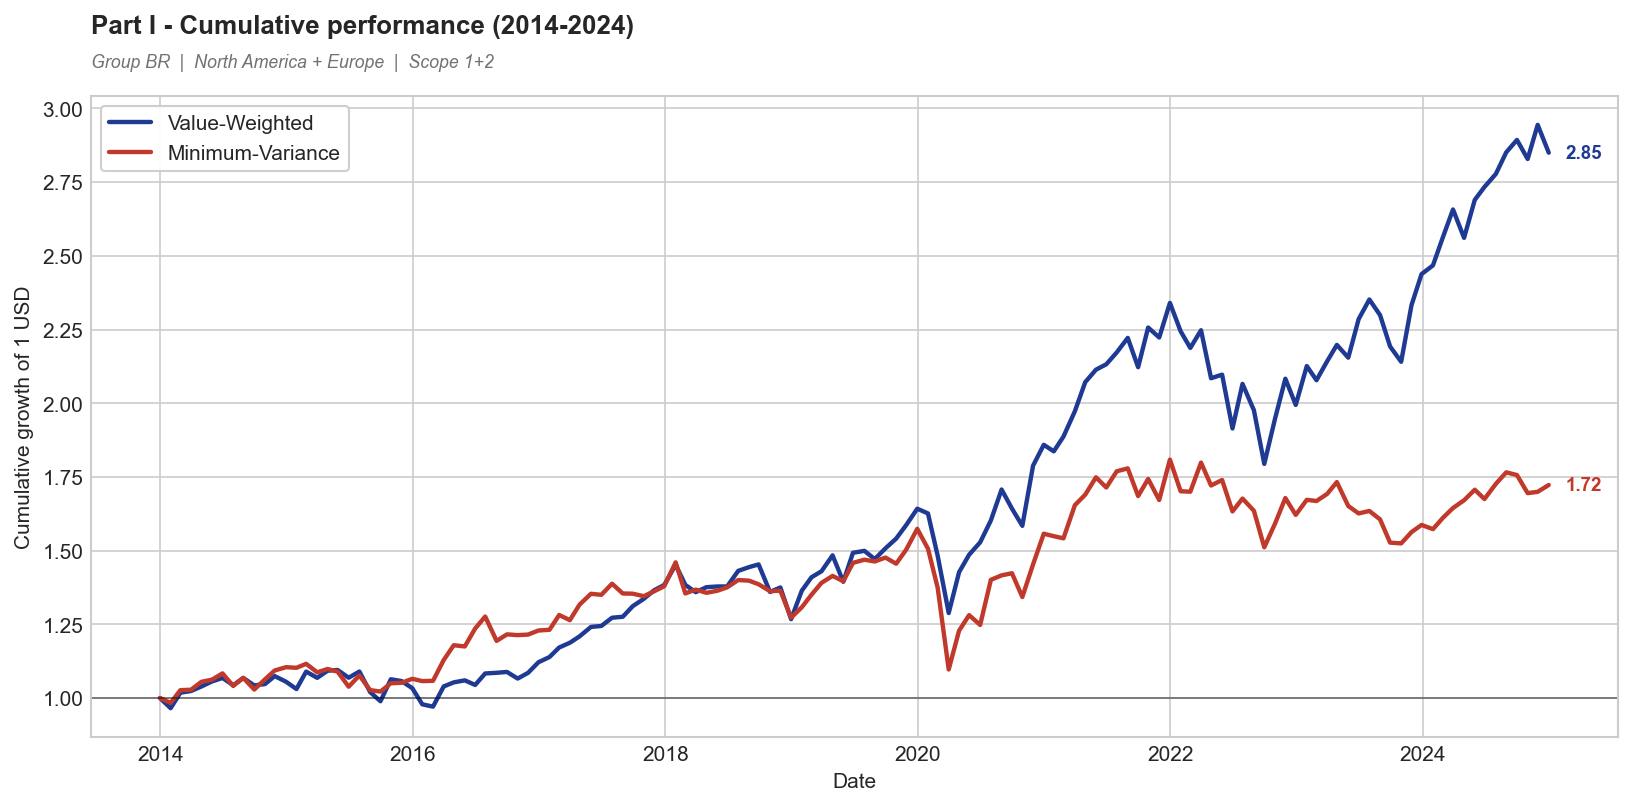
\includegraphics[width=0.92\textwidth]{cum_part1.png}
\caption{\textbf{Cumulative performance of the Part I portfolios.} Growth of one
dollar invested in January 2014, plotted month by month to December 2024 (the
series start at 1). The minimum-variance portfolio is more defensive in
2014--2018 but falls sharply in the March 2020 crash and never recovers the gap,
illustrating that low-volatility investing lagged badly in a sustained bull
market.}
\label{fig:part1}
\end{figure}

Two features deserve comment. First, the minimum-variance portfolio reduces
realised volatility only marginally (14.04\% versus 14.62\%) -- far less than its
\emph{estimated} variance would suggest. With about 1{,}000 firms and only 120
monthly observations, the sample covariance matrix is severely
rank-deficient and noisy; the optimiser exploits estimation error, concentrating
in roughly 34 names (effective number of holdings $\approx 17$) whose
\emph{past} variance was low but whose \emph{future} variance was not. Its worst
month ($-20.2\%$) is in fact deeper than the benchmark's. Second, the
defensive style underperformed: over 2014--2024 low-volatility stocks lagged the
mega-cap growth names that drove the cap-weighted index. Both observations are a
direct consequence of the prescribed estimator and are revisited in
Section~\ref{sec:limits}.

% ================================================================ 5
\section{Part II -- Carbon Profile of the Base Portfolios (\S3.1)}

Before decarbonising, we measure the carbon profile of the two Part~I
portfolios. Figure~\ref{fig:carbonbase} shows the weighted-average carbon
intensity and the carbon footprint of \pvw{} and \pmv{} for every allocation
year.

\begin{figure}[H]
\centering
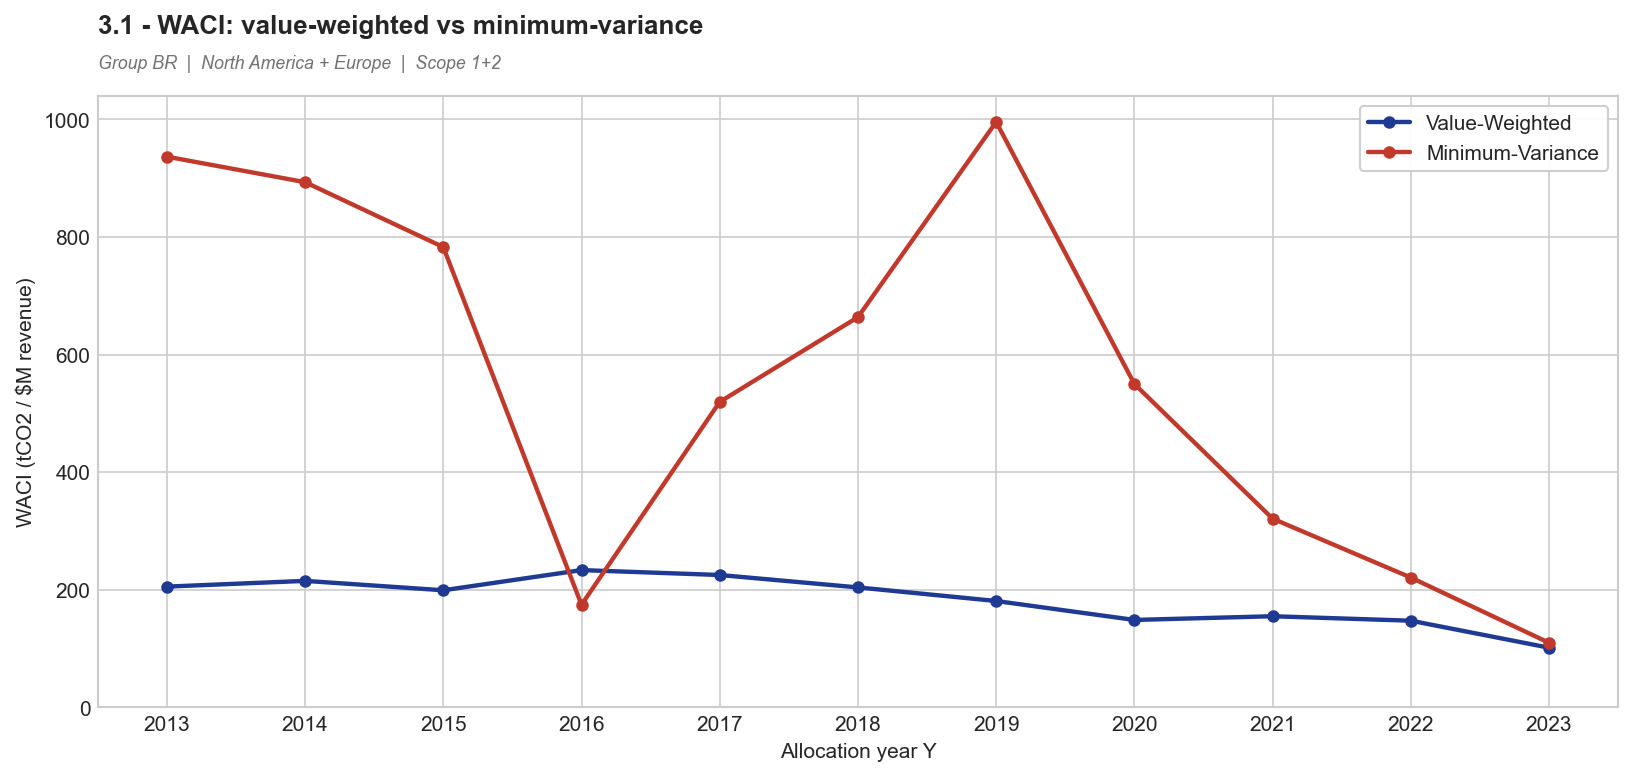
\includegraphics[width=0.80\textwidth]{waci_base.png}\\[4pt]
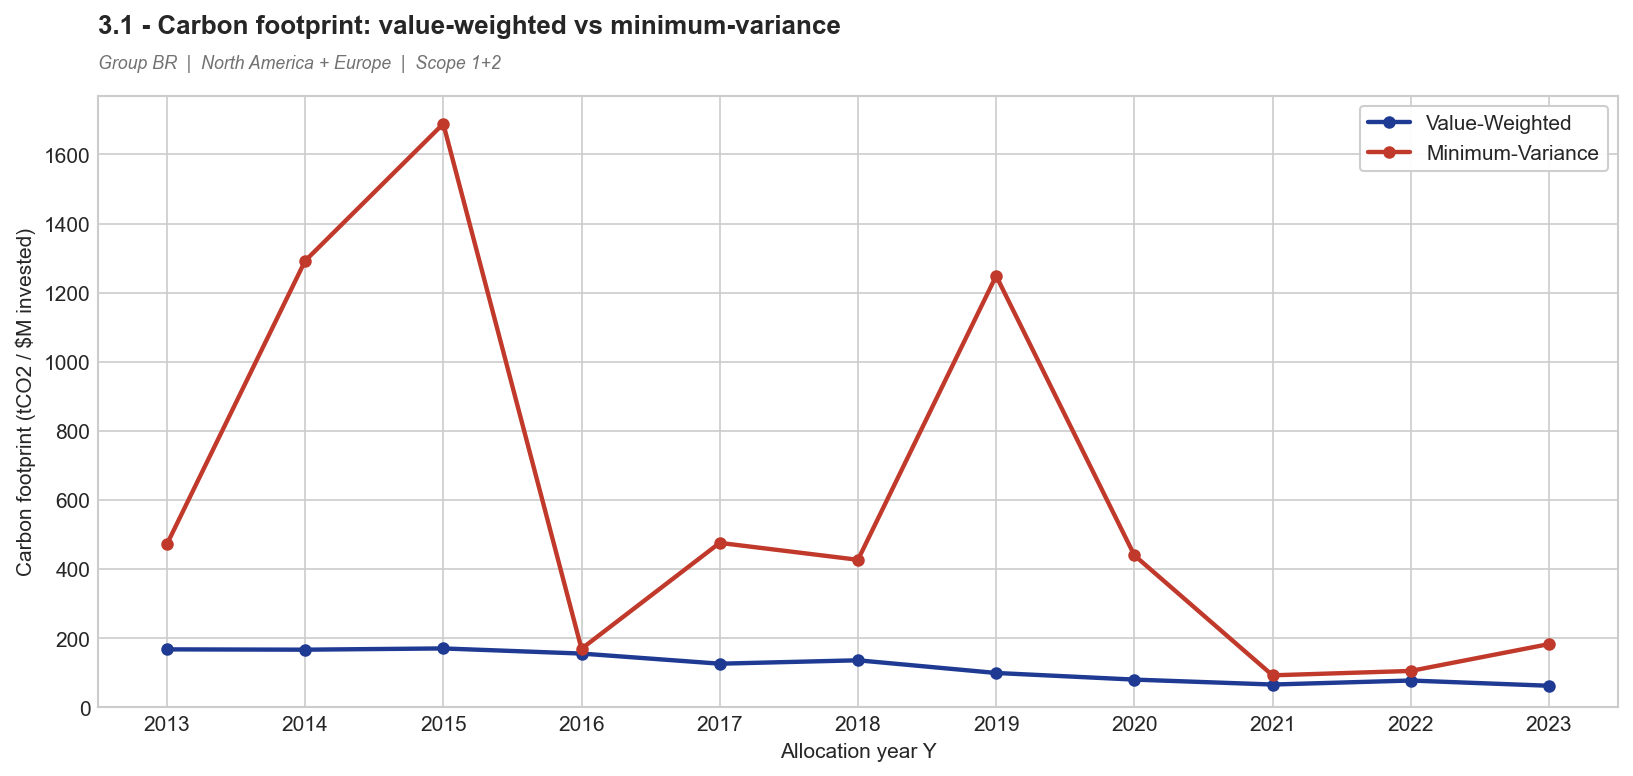
\includegraphics[width=0.80\textwidth]{cf_base.png}
\caption{\textbf{Carbon profile of the value-weighted and minimum-variance
portfolios.} Top: weighted-average carbon intensity (WACI, tonnes \co{} per
million USD of revenue). Bottom: carbon footprint (CF, tonnes \co{} per million
USD invested). Both are computed from the allocation weights and the Scope~1+2
emissions of year $Y$. The benchmark decarbonises steadily; the
minimum-variance portfolio is far more carbon-intensive and extremely unstable
from one year to the next.}
\label{fig:carbonbase}
\end{figure}

The benchmark's footprint declines markedly, from 167.8 in 2013 to 62.5 in 2023
(WACI from 205 to 101). This reflects both genuine corporate decarbonisation and
a compositional drift of the cap-weighted universe toward low-carbon mega-cap
technology firms. The minimum-variance portfolio tells the opposite story: its
average footprint, 599.6, is \textbf{five times} the benchmark's (119.1), and it
swings violently -- from about 170 to nearly 1{,}700 tonnes per million USD
across years. The economic explanation is important: the minimum-variance
optimiser favours low-volatility stocks, and in this universe the lowest-beta
names are regulated electric utilities, whose emissions per dollar of market
value are very large. \emph{An investor who minimises variance unknowingly takes
a massive, unstable carbon overweight.} This is the central motivation for
Part~II.

\paragraph{Who drives the intensity up?} Table~\ref{tab:top10} ranks the ten
largest contributors to the benchmark's WACI. The list is dominated by US
electric utilities (Duke Energy, Southern, NextEra, American Electric Power,
Dominion, Xcel), complemented by a cement producer (Holcim) and the two
integrated oil majors (ExxonMobil, Chevron). Utilities and cement combine a high
carbon intensity with a non-trivial index weight; the oil majors have a lower
intensity per dollar of \emph{revenue} but enter the list through their large
benchmark weight. These names are the natural targets of the carbon constraint.

\begin{table}[H]
\centering
\caption{\textbf{Top-10 contributors to the benchmark's carbon intensity.}
Firms ranked by their average contribution $\alpha^{(vw)}_{i,Y}\,CI_{i,Y}$ to the
value-weighted WACI over 2013--2023. ``CI 2023'' is the firm's carbon intensity
in the last allocation year and ``VW weight'' its benchmark weight then. A large
contribution comes either from a very high intensity (utilities, cement) or from
a large weight (oil majors).}
\label{tab:top10}
\small
\begin{tabular}{lllrrr}
\toprule
Firm & ISIN & Country & \makecell{Avg WACI\\contrib.} &
\makecell{CI 2023} & \makecell{VW weight\\2023 (\%)}\\
\midrule
Duke Energy            & US26441C2044 & US & 9.51 & 2552.6 & 0.16\\
Southern               & US8425871071 & US & 8.92 & 2717.7 & 0.16\\
NextEra Energy         & US65339F1012 & US & 7.80 & 2018.3 & 0.27\\
American Elec.\ Power   & US0255371017 & US & 6.22 & 2269.1 & 0.09\\
Dominion Energy        & US25746U1097 & US & 5.17 & 1744.9 & 0.08\\
Holcim                 & CH0012214059 & CH & 5.03 & 2430.9 & 0.10\\
ExxonMobil             & US30231G1022 & US & 4.69 & \phantom{0}250.8 & 0.85\\
Air Products \& Chem.   & US0091581068 & US & 3.79 & 2143.0 & 0.13\\
Xcel Energy            & US98389B1008 & US & 3.55 & 2383.4 & 0.07\\
Chevron                & US1667641005 & US & 3.23 & \phantom{0}229.1 & 0.60\\
\bottomrule
\end{tabular}
\end{table}

\begin{figure}[H]
\centering
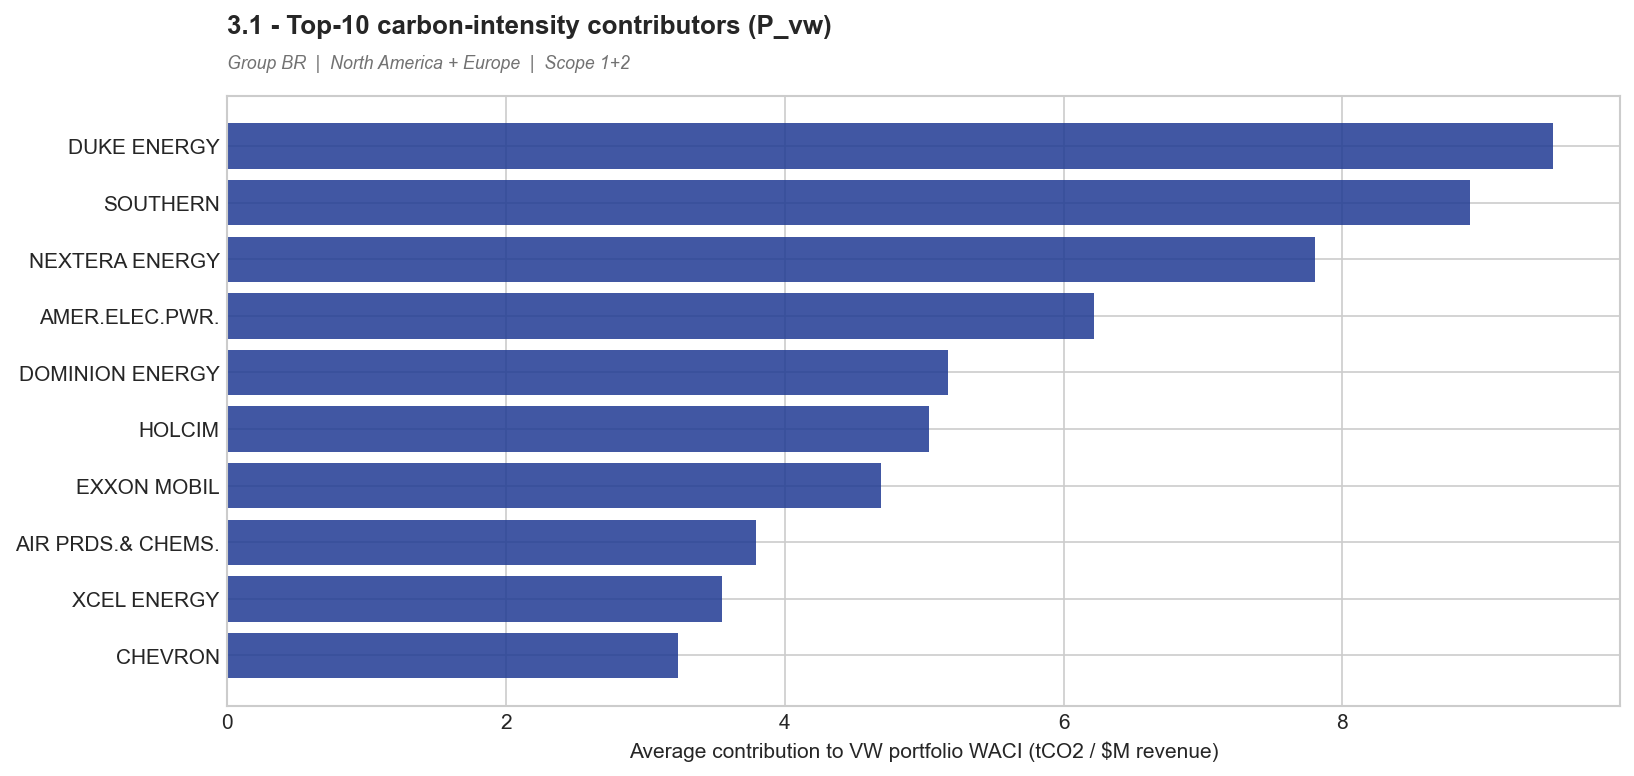
\includegraphics[width=0.86\textwidth]{top10_emitters.png}
\caption{\textbf{Top-10 carbon-intensity contributors of the benchmark.} Bar
length is the average contribution to the value-weighted WACI over 2013--2023.
Removing or under-weighting this short list of names accounts for most of the
achievable decarbonisation.}
\label{fig:top10}
\end{figure}

% ================================================================ 6
\section{Part II -- Decarbonised Portfolios}

\subsection{Minimum variance with a 50\% footprint cut: \pmvh{} (\S3.2)}

\pmvh{} re-solves the minimum-variance problem with the footprint capped at
half of \pmv{}'s footprint each year. Because the footprint constraint is
linear, the cap binds exactly: \pmvh{} achieves precisely 50\% of \pmv{}'s
footprint every year (Figure~\ref{fig:mv05}, bottom). The remarkable result is
the \emph{financial} side (Table~\ref{tab:full}): halving the carbon footprint
\textbf{improves} the portfolio. Annualised volatility falls from 14.04\% to
13.03\%, the Sharpe ratio rises from 0.42 to 0.46, and the worst month
improves from $-20.2\%$ to $-17.8\%$.

\begin{figure}[H]
\centering
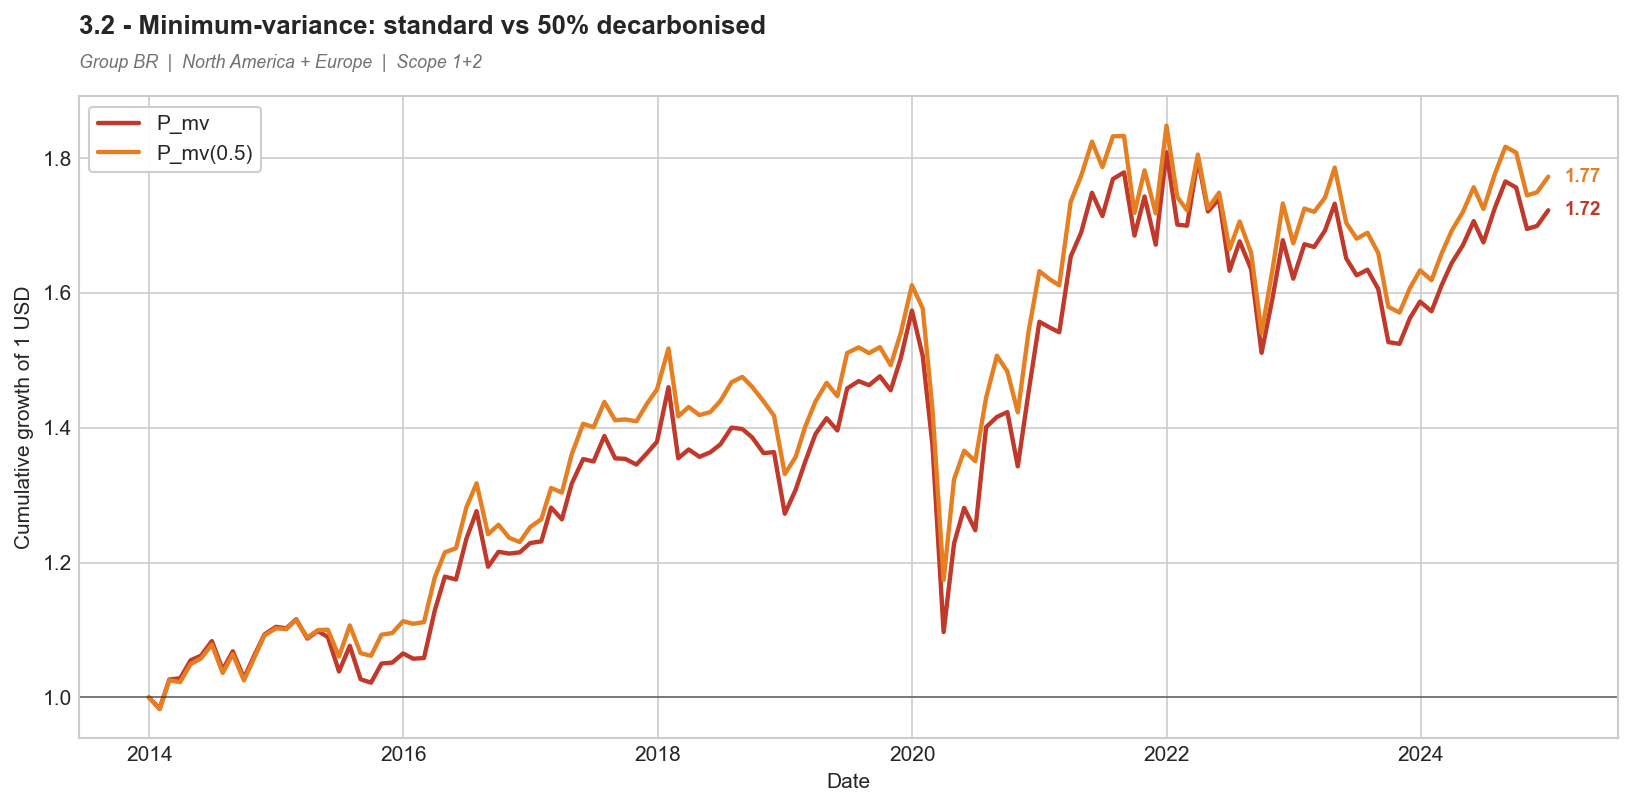
\includegraphics[width=0.80\textwidth]{cum_mv05.png}\\[4pt]
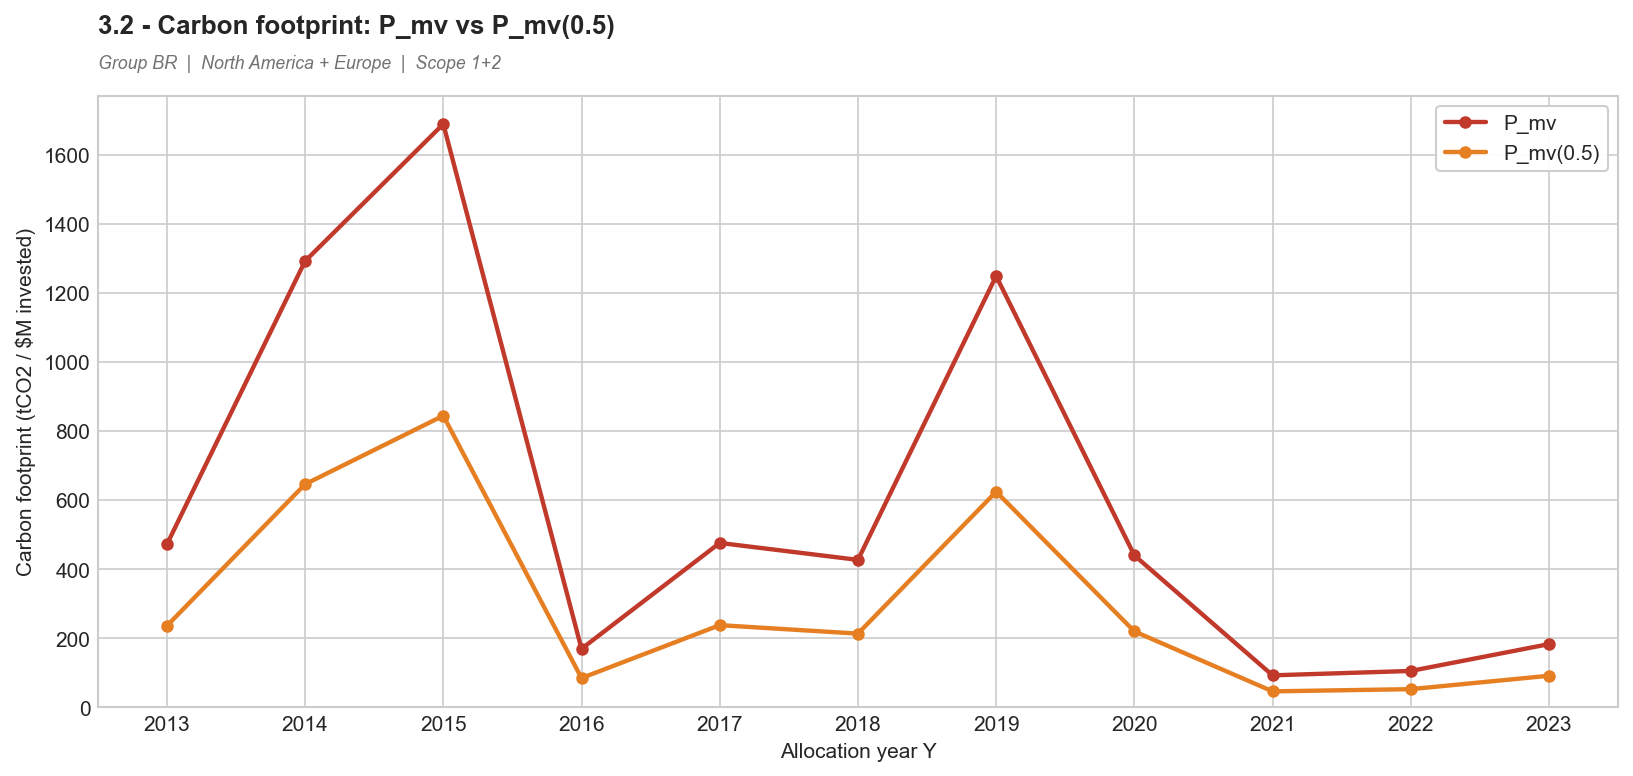
\includegraphics[width=0.80\textwidth]{cf_mv05.png}
\caption{\textbf{Decarbonising the minimum-variance portfolio.} Top: cumulative
growth of one dollar, \pmv{} versus \pmvh{}. Bottom: carbon footprint by
allocation year. The 50\% cap binds exactly every year; the decarbonised
portfolio nevertheless ends \emph{above} the standard one, because the carbon
constraint forces the optimiser away from concentrated, carbon-heavy utility
bets that also turned out to be risky.}
\label{fig:mv05}
\end{figure}

The intuition is that the carbon constraint and good risk management point in
the same direction here. The high-carbon utility names that \pmv{} loads on are
also the concentrated, estimation-error-driven positions; capping the footprint
disperses weight toward a broader set of low-volatility firms, which both
lowers realised risk and removes the carbon overweight. Decarbonisation is not
merely free for the active minimum-variance investor -- it is mildly beneficial.

\subsection{Tracking-error minimisation with a 50\% cut: \pvwh{} (\S3.3)}

\pvwh{} is the ``otherwise passive'' strategy: stay as close as possible to the
benchmark while halving its footprint. Table~\ref{tab:full} shows that this is
inexpensive. The annualised return slips from 10.62\% to 10.16\%, the Sharpe
ratio from 0.72 to 0.69, and the annualised ex-post tracking error is only
1.1\%. The footprint is cut by 50\% on average (59.2 versus 119.1), and in fact
slightly more than 50\% in most years (Figure~\ref{fig:vw05}, bottom): the
tracking-error objective is flat in the directions spanned by the covariance
matrix's null space, so the optimiser comfortably reaches -- and marginally
over-shoots -- the carbon ceiling at no additional tracking cost.

\begin{figure}[H]
\centering
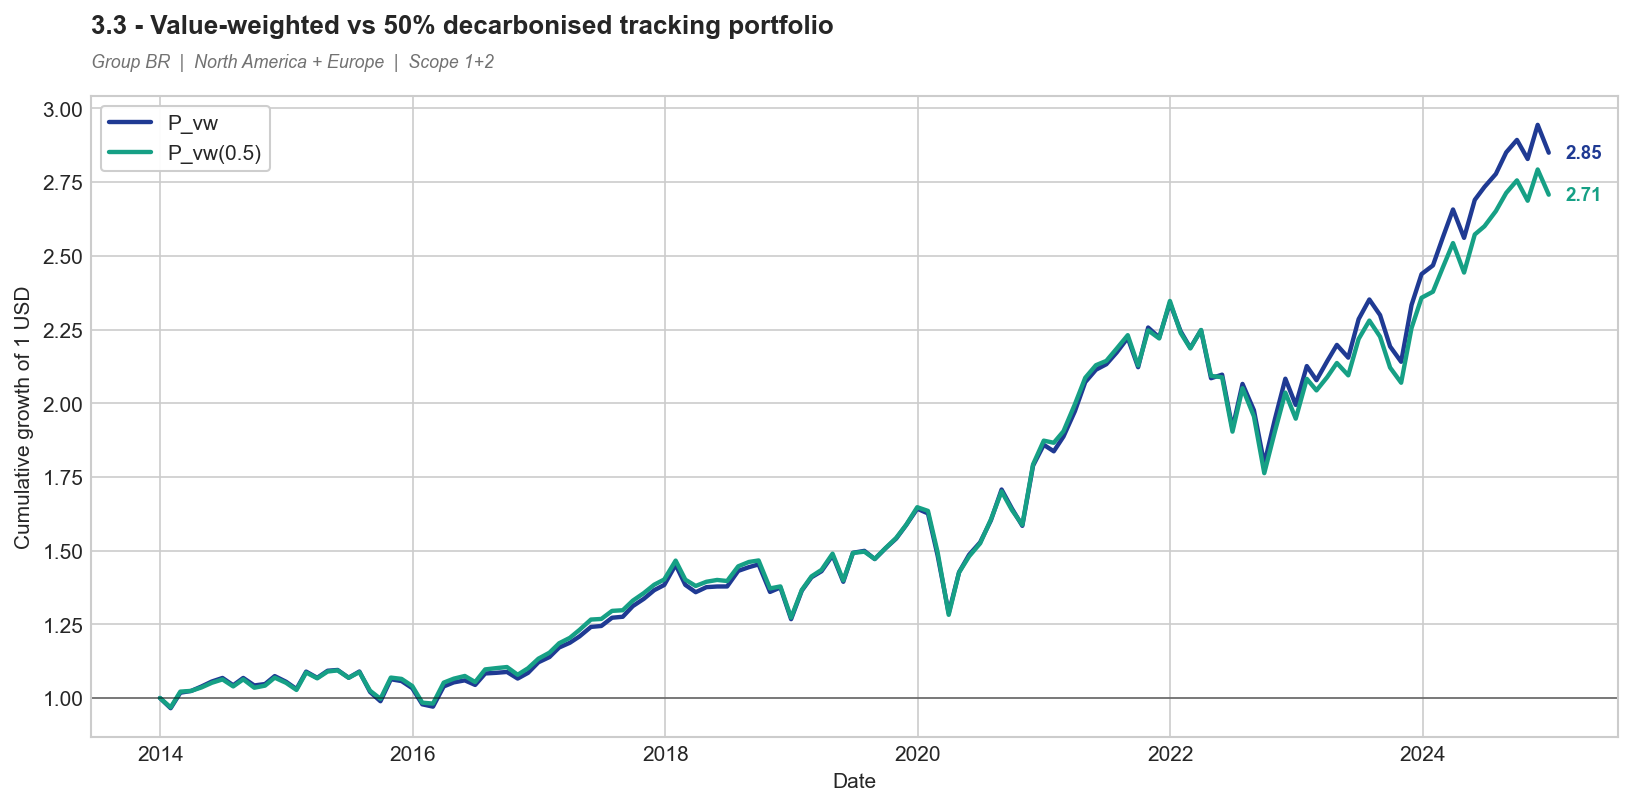
\includegraphics[width=0.80\textwidth]{cum_vw05.png}\\[4pt]
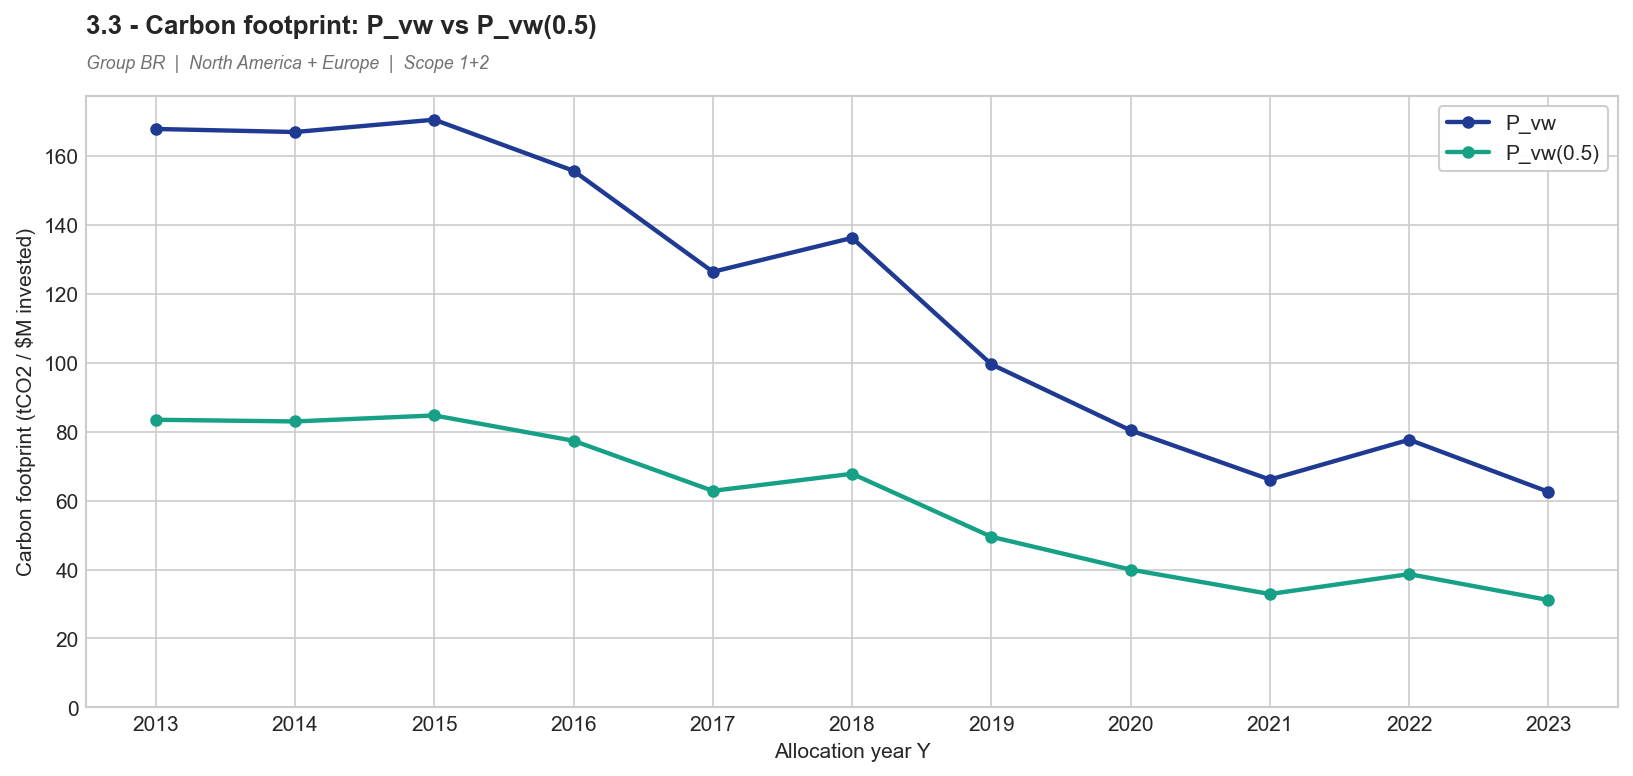
\includegraphics[width=0.80\textwidth]{cf_vw05.png}
\caption{\textbf{Decarbonising the benchmark through a tracking overlay.} Top:
cumulative growth of one dollar, \pvw{} versus \pvwh{}. Bottom: carbon
footprint. The two return paths are visually almost indistinguishable
(annualised tracking error 1.1\%) while the footprint is permanently halved.}
\label{fig:vw05}
\end{figure}

Because the constraint removes only a short list of high-intensity names
(Table~\ref{tab:top10}) that carry little of the benchmark's overall risk, the
portfolio can be rebuilt from the remaining $\approx$~980 firms with almost no
tracking cost. The country composition barely moves: at the 2023 rebalancing,
\pvwh{} trims the United States by about 2~percentage points and France by
1~point, and tilts modestly toward the United Kingdom, Sweden and Israel --
small rotations away from utility- and energy-heavy markets.

\subsection{Comparison of \pmv/\pmvh{} and \pvw/\pvwh{} (\S3.4)}

The two decarbonisation exercises reveal a clear pattern. For the
\textbf{active} minimum-variance investor, the footprint cut reshapes a
concentrated portfolio and happens to improve it; the ``cost'' of carbon is
negative here, but the portfolio remains far from the benchmark (tracking error
8.8\%) and still carries an above-market footprint (299.8, because 50\% of a very
large number is still large). For the \textbf{passive} investor, the footprint
cut is a genuine constraint -- the unconstrained optimum is the benchmark itself
-- yet its cost is tiny (0.03 of Sharpe ratio) and the resulting footprint, 59.2,
is the lowest of all five portfolios. The lesson is that \emph{where} the carbon
constraint is applied matters: a decarbonisation overlay on a well-diversified
benchmark is far more efficient than decarbonising an already-concentrated
optimised portfolio.

\subsection{Net-zero portfolio: \pnz{} (\S4)}

\pnz{} keeps the tracking-error objective but replaces the fixed 50\% cap with a
glide path: the footprint ceiling falls by 10\% per year relative to the 2013
benchmark footprint, reaching $(1-0.10)^{11}\approx 31\%$ of it by the last
allocation. Figure~\ref{fig:netzero} shows that the portfolio tracks the glide
path closely every year; all targets remain feasible over the sample.

\begin{figure}[H]
\centering
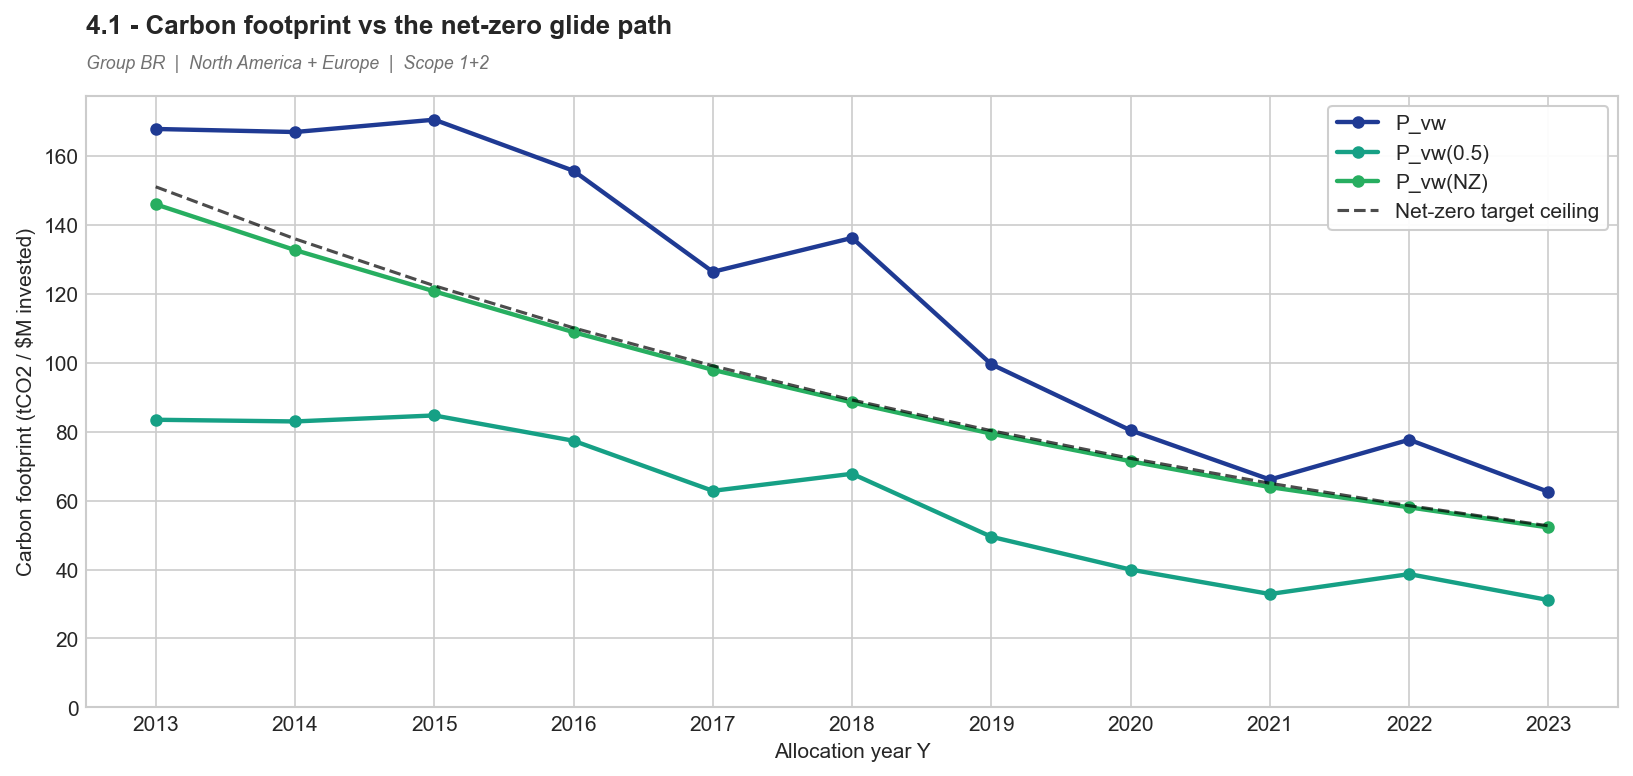
\includegraphics[width=0.80\textwidth]{cf_netzero.png}\\[4pt]
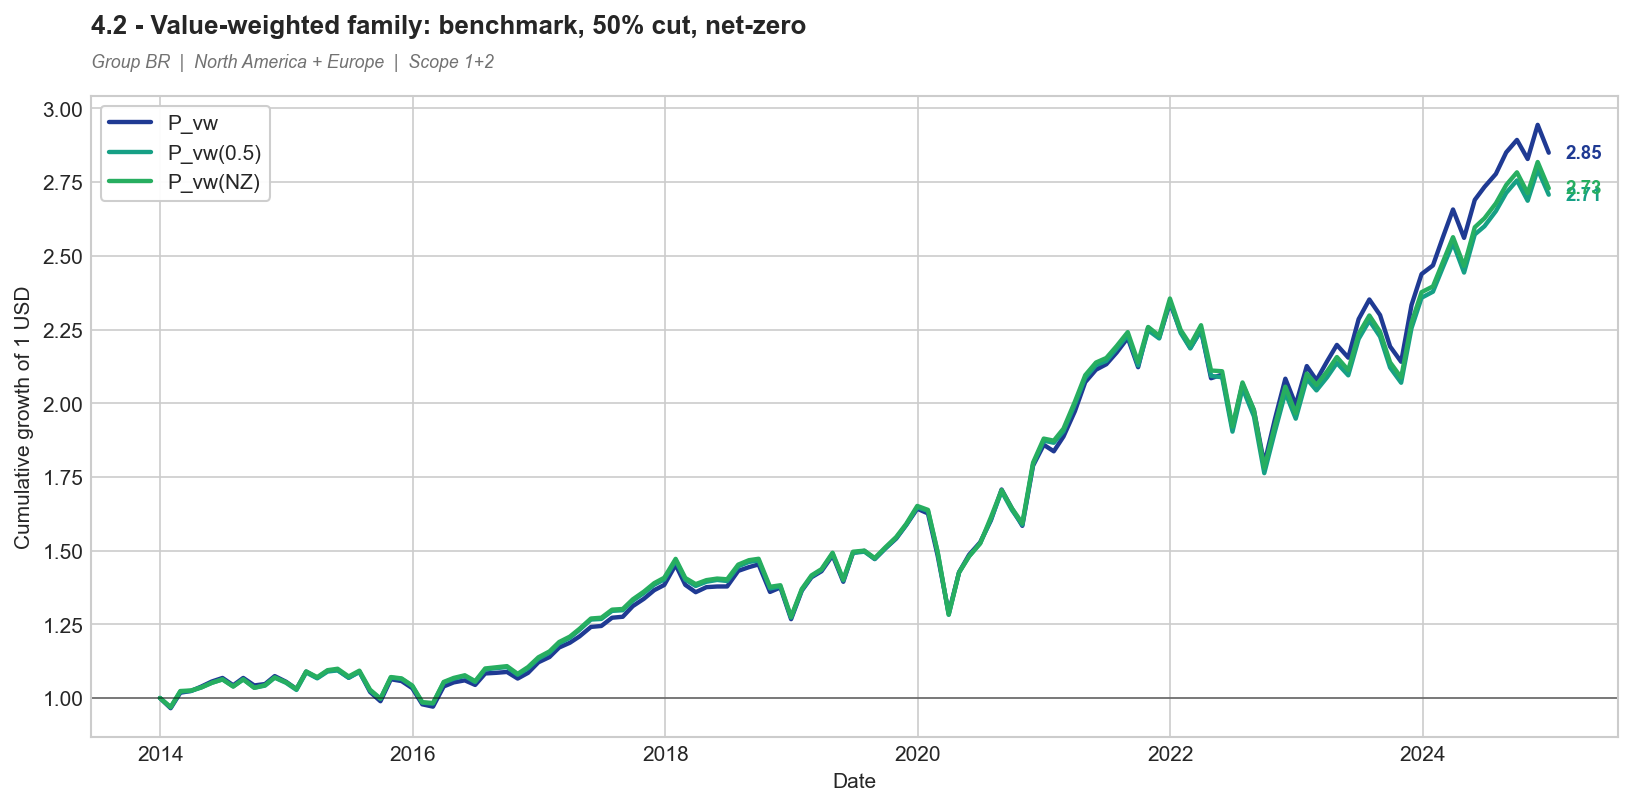
\includegraphics[width=0.80\textwidth]{cum_netzero.png}
\caption{\textbf{The net-zero portfolio.} Top: carbon footprint of \pvw{},
\pvwh{} and \pnz{} against the 10\%-per-year glide path (dashed). \pnz{} hugs the
ceiling; the fixed-50\% portfolio \pvwh{} is actually lower in later years,
because ``50\% of the contemporaneous benchmark'' becomes more demanding than a
path anchored to 2013 once the benchmark has decarbonised on its own. Bottom:
cumulative growth of one dollar -- the three value-weighted-family portfolios
are nearly indistinguishable.}
\label{fig:netzero}
\end{figure}

Financially, \pnz{} costs about the same as the one-off 50\% cut: a Sharpe ratio
of 0.69 and an annualised tracking error of 1.1\% (Table~\ref{tab:full}). Its
\emph{average} footprint over the sample, 92.7, is higher than \pvwh{}'s 59.2,
which looks paradoxical for a ``net-zero'' strategy. The reason is the anchoring:
the glide path is fixed to the 2013 level, but the benchmark itself decarbonised
by more than 60\% over the decade, so by 2023 the cumulative
$-69\%$ target translates into only about $-16\%$ relative to the
\emph{contemporaneous} benchmark. A genuinely demanding net-zero design should
either anchor the glide path to a rolling benchmark or combine the cumulative
rule with a ``50\% of current'' floor.

\begin{table}[H]
\centering
\caption{\textbf{Consolidated comparison of all five portfolios
(Jan 2014 -- Dec 2024).} Annualised performance statistics, ex-post tracking
error against the benchmark, sample-average carbon footprint and WACI, the
footprint change relative to \pvw{}, and the average effective number of
holdings $N_{\text{eff}}=1/\sum_i\alpha_i^2$. Carbon figures are in tonnes \co{}
per million USD (invested for CF, of revenue for WACI). Lower CF/WACI and higher
Sharpe are better; a low tracking error means the portfolio stays close to the
benchmark.}
\label{tab:full}
\small
\renewcommand{\arraystretch}{1.15}
\begin{tabular}{lccccc}
\toprule
 & \pvw{} & \pmv{} & \pmvh{} & \pvwh{} & \pnz{}\\
\midrule
Annualised avg return        & 10.62\% & 5.96\%  & 6.07\%  & 10.16\% & 10.23\%\\
Annualised volatility        & 14.62\% & 14.04\% & 13.03\% & 14.63\% & 14.64\%\\
Annualised cumulative return & \phantom{0}9.99\% & 5.07\% & 5.34\% & \phantom{0}9.48\% & \phantom{0}9.56\%\\
Sharpe ratio                 & 0.72 & 0.42 & 0.46 & 0.69 & 0.69\\
Minimum monthly return       & $-13.1\%$ & $-20.2\%$ & $-17.8\%$ & $-14.2\%$ & $-14.2\%$\\
Maximum monthly return       & 12.9\% & 12.3\% & 12.7\% & 12.9\% & 12.9\%\\
Annualised tracking error    & --   & 9.66\% & 8.84\% & 1.09\% & 1.13\%\\
\midrule
Avg carbon footprint (CF)    & 119.1 & 599.6 & 299.8 & 59.2 & 92.7\\
Avg carbon intensity (WACI)  & 183.2 & 560.6 & 255.6 & 90.7 & 130.3\\
CF vs \pvw{}                 & --   & $+404\%$ & $+152\%$ & $-50\%$ & $-22\%$\\
Avg effective \# holdings    & 159 & 17 & 18 & 158 & 161\\
\bottomrule
\end{tabular}
\end{table}

% ================================================================ 7
\section{Discussion: the Cost of Decarbonisation}

The headline finding is that, over this sample and universe, decarbonisation is
\textbf{close to free for a passive investor and mildly profitable for an active
minimum-variance investor}. Three mechanisms explain this.

First, the carbon footprint is highly concentrated. A handful of utilities,
plus cement and oil, account for most of the benchmark's intensity
(Table~\ref{tab:top10}). Cutting the footprint therefore requires re-weighting
only a small slice of the portfolio, and the broad diversified core is left
untouched -- hence the 1.1\% tracking error of \pvwh{} and \pnz{}.

Second, decarbonising and de-risking are aligned for the minimum-variance
investor. The carbon-heavy utilities that \pmv{} over-weights are exactly its
concentrated, fragile positions; the carbon cap disperses them and lowers
realised volatility.

Third, the benchmark decarbonised on its own. The value-weighted footprint fell
by more than 60\% over 2013--2023 as the index rotated toward low-carbon
technology leaders. This makes any glide path anchored to 2013 progressively
easier to satisfy and is the reason \pnz{} ends up less aggressive than the
fixed-50\% rule.

These conclusions are sample-specific. The 2014--2024 decade was a long bull
market in which low-carbon technology names happened to be the best performers.
In a regime where energy and materials lead -- as in 2022 -- a carbon constraint
would create a real performance drag. The figures here should be read as the
cost of decarbonisation \emph{in a favourable climate-transition regime}, not as
a universal free lunch.

% ================================================================ 8
\section{Robustness Checks and Suggested Improvements}

The following extensions would strengthen the analysis:
\begin{itemize}[nosep,leftmargin=1.3em]
  \item \textbf{Better covariance estimation.} Replace the raw sample
        covariance with Ledoit--Wolf shrinkage or a factor model. This would
        most affect \pmv{} and \pmvh{}, whose concentration is an artefact of
        estimation error, and is the single most valuable improvement.
  \item \textbf{Missing-return treatment.} Setting missing returns to zero
        biases variances downward for sparsely-covered firms. Restricting the
        universe to firms with near-complete return histories, or using
        pairwise / EM covariance estimation, would test the sensitivity of the
        minimum-variance results.
  \item \textbf{Parameter sensitivity.} Re-run the back-test for stale-price
        thresholds of 30\%/70\%, minimum-observation counts of 24/60, and
        estimation windows of 5/7~years, and report how the Sharpe ratio and
        footprint move.
  \item \textbf{Transaction costs and turnover.} Add realistic trading costs
        and measure annual turnover; the carbon-constrained portfolios may
        trade more as the high-intensity name list changes year to year.
  \item \textbf{Footprint denominator.} Recompute CF using enterprise value
        including cash (EVIC) instead of market capitalisation, the current
        EU-regulation standard, to remove the mechanical sensitivity of the
        footprint to equity valuations.
  \item \textbf{Diversification controls.} Add a maximum-weight cap (e.g.\ 5\%)
        to the minimum-variance problem to curb its concentration directly, and
        compare with the carbon-constrained version.
\end{itemize}

% ================================================================ 9
\section{Limitations}
\label{sec:limits}

\begin{itemize}[leftmargin=1.5em]
  \item \textbf{Data quality.} Carbon coverage is thin before 2010 and the 2024
        reporting year is still incomplete (about 1{,}950 firms reported versus
        2{,}260 in 2023); forward-filling propagates stale figures. Scope~1+2
        emissions are self-reported with non-uniform methodology, and Scope~3 --
        often the largest perimeter -- is excluded entirely.
  \item \textbf{Estimation issues.} A 120-month covariance matrix for
        $\approx$~1{,}000 firms is severely rank-deficient. The minimum-variance
        portfolio exploits this noise and concentrates in $\approx$~17 effective
        names; its footprint consequently swings between 170 and 1{,}700 tonnes
        per million USD across adjacent years.
  \item \textbf{Parameter sensitivity.} Results depend on several discretionary
        choices -- the 50\% stale-price threshold, the 36-observation minimum,
        the 10-year window, the $10^{-8}$ ridge -- none of which is formally
        optimised. The minimum-variance family is the most exposed to these
        choices.
  \item \textbf{Constraint feasibility.} All carbon targets are feasible over
        2013--2023, but a long-only, fully-invested portfolio cannot push its
        footprint below $\min_i E_{i,Y}/Cap_{i,Y}$. A net-zero glide path
        extended far enough, or anchored to a rolling benchmark, would
        eventually become infeasible without short positions, carbon offsets or
        a cash allocation.
  \item \textbf{Carbon-metric design.} The footprint uses market capitalisation
        in the denominator, so a market sell-off mechanically raises measured
        intensity even when real emissions are unchanged; conclusions are also
        regime-dependent (a fossil-led market would reverse the ``free lunch'');
        and the absence of sector identifiers in the dataset means sector tilts
        can only be proxied through country and firm-level composition.
\end{itemize}

% ================================================================ 10
\section{Conclusion}

On a North American and European equity universe, we constructed a
value-weighted benchmark, a minimum-variance portfolio and three decarbonised
variants, back-tested monthly over 2014--2024. The minimum-variance portfolio
underperformed the benchmark and -- contrary to a naive expectation -- carried a
carbon footprint several times larger, because low-volatility investing is an
implicit overweight of carbon-heavy regulated utilities. Imposing a carbon
constraint corrected this at negligible cost: a tracking-error overlay halved
the benchmark's footprint for 0.03 of Sharpe ratio and a 10\%-a-year
net-zero glide path cost barely more, while decarbonising the minimum-variance
portfolio actually improved its risk-adjusted return. The efficiency of
decarbonisation depends critically on \emph{how} it is implemented -- as a light
overlay on a diversified benchmark rather than a constraint on an already
concentrated portfolio -- and on a market regime that, over this decade,
rewarded the low-carbon transition.

\end{document}
